\documentclass[10pt]{article}
\usepackage[margin=1in]{geometry}
\usepackage{graphicx}
\usepackage{booktabs}
\usepackage{url}
\usepackage{amsmath}
\usepackage{siunitx}
\usepackage[hidelinks]{hyperref}
\graphicspath{{../figures/}}

\title{HBM-PIM Phase 1: ECC Reporting, Output Control, Pause and Recovery}
\author{Phase 1 Experimental Framework}
\date{2026-11-16}

\begin{document}
\maketitle

\begin{abstract}
We implement and execute a model study of ECC observability, host/device output
control, channel quiescence, trusted-input recovery and fault-free cost for an
HBM-PIM ADD kernel. The study uses the fixed PIMSimulator commit
\texttt{3703d1f19c8f027360cc33a3243eb271e3bb6898}. It is a model study: the
ECC layout, control interface and notification path are explicit assumptions,
not measurements of a commercial product. The paper matrix contains 2602 cases;
2595 succeed, 7 are expected negatives, and none fail or time out. A separate
supplement adds 4650 constructed-escape and report-sequence cases; all 4650
succeed, with no failure, timeout or missing case.
\end{abstract}

\section{Scope and platform}
The platform is a single HBM2 PIM model with 16 banks, one rank, FP16 and
Scheme8 addressing. The producer is $B=A+X$; a PIM consumer optionally executes
$C=B\times2$. We compare four model profiles: NATIVE, LOCAL\_VISIBLE,
LOCAL\_HIDDEN and HOST\_ONLY. LOCAL\_VISIBLE is the main profile. The ECC is a
research SECDED(72,64) model with four codewords per 32\,B burst. The runtime
sees only the public fields \texttt{report\_seq}, \texttt{report\_cycle},
\texttt{error\_class}, \texttt{region\_type} and \texttt{region\_id}; it does
not read \texttt{truth.csv} or a reference output.

The supplement asks two further questions. P1-G constructs ECC escapes
(miscorrection F3M, silent F4S, and a CE witness plus silent F4S) and tests
whether timely control withholds an actually corrupted output. P1-H compares
multi-report sequences under bank, page and an ASSUMED codeword granularity,
with and without an ASSUMED idealized scrub, to test what coarse public reports
can distinguish. The supplement has an independent manifest with 4320 P1-G and
330 P1-H cases (4650 total) and is not counted in the 2602 paper cases.

\section{Method}
For every W1 case, C++ and an independent Python/NumPy reference generate the
same inputs. Final B bytes are compared exactly; W2 compares $(A+X)\times2$ in
the same FP16 order. Continuous summaries use seed-level means and 95\%
bootstrap intervals (10000 resamples, statistic seed 20261115). Binary
proportions use Wilson 95\% intervals. A 30-seed 100\% result has a Wilson lower
bound of 88.6\%, so zero observed failures is not presented as a population
guarantee.

\section{Results}

\subsection{Protection paths}
Table~\ref{tab:paths} summarizes the F1 path-coverage panel of Fig.~\ref{fig:path}.
LOCAL\_VISIBLE and LOCAL\_HIDDEN correct all four paths; only LOCAL\_VISIBLE
delivers CE. HOST\_ONLY corrects the host path but exposes the PIM path gap.
NATIVE neither corrects nor reports. F2 same-codeword errors are UE for the
protected profiles and are not counted as recovered output.

\begin{table}[t]
\centering
\caption{F1 single-bit correctness and report delivery (3 banks per cell).}
\label{tab:paths}
\begin{tabular}{lcccc}
\toprule
profile & HREAD & PREAD & PWRITE\_HREAD & PWRITE\_PREAD \\
\midrule
NATIVE & 0/3 & 0/3 & 0/3 & 0/3 \\
LOCAL\_VISIBLE & 3/3 C, 3 R & 3/3 C, 3 R & 3/3 C, 3 R & 3/3 C, 3 R \\
LOCAL\_HIDDEN & 3/3 C, 0 R & 3/3 C, 0 R & 3/3 C, 0 R & 3/3 C, 0 R \\
HOST\_ONLY & 3/3 C, 3 R & 0/3 & 0/3 & 0/3 \\
\bottomrule
\end{tabular}
\end{table}

\begin{figure}[t]
\centering
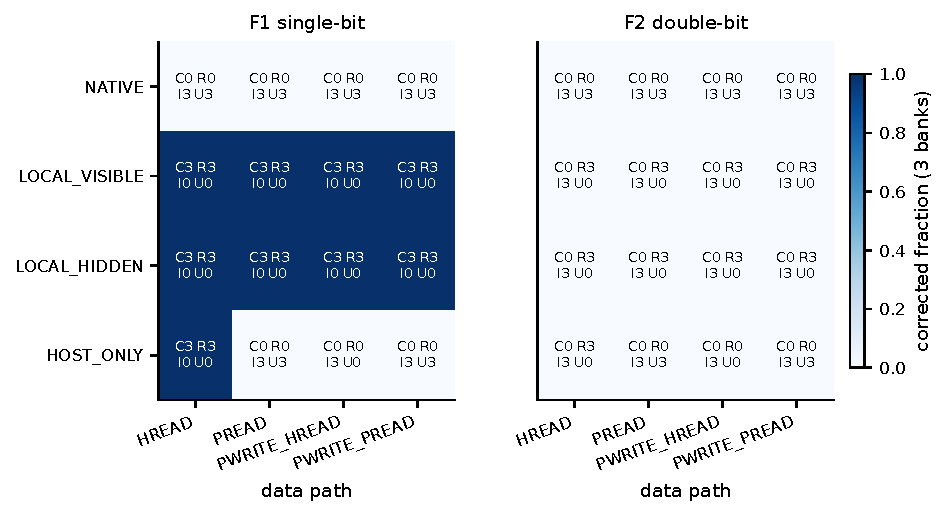
\includegraphics[width=\linewidth]{fig01_path_coverage.pdf}
\caption{Path coverage. Cell labels are C corrected, R reported, I invalid and
U uncovered counts over three banks; color is corrected fraction. F1 and F2
are separate panels. The profiles are model behaviors, not product claims.}
\label{fig:path}
\end{figure}

\subsection{Report latency and location}
A single W0/HREAD event has observed latency 1 cycle at D=0 or D=1, and
16/256/4096 cycles at D=16/256/4096. The 32-read burst at I=8 delivers all 32
CE reports without drops, with FIFO order, at least 8 cycles between reports,
and the expected bank/page identity. Fig.~\ref{fig:latency} also shows the
cumulative burst delivery; matching the configured delay validates the model,
not a hardware latency.

\begin{figure}[t]
\centering
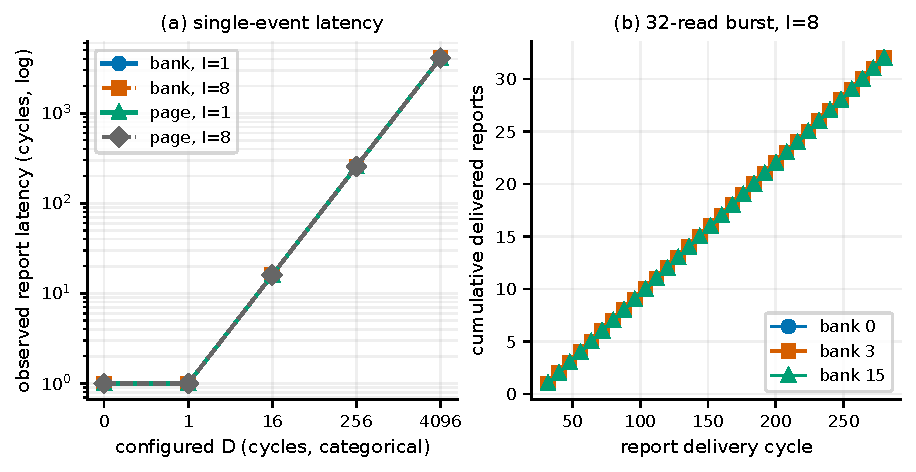
\includegraphics[width=\linewidth]{fig02_report_latency.pdf}
\caption{(a) Single-event notification latency versus configured D; D=0 is a
separate category and the y axis is logarithmic. (b) Cumulative burst reports
for three banks at I=8.}
\label{fig:latency}
\end{figure}

\subsection{Control window}
The main P1-C matrix has 1800 LOCAL\_VISIBLE cases: 30 seeds, two tile counts,
two consumers, five $D/T_{\mathrm{ref}}$ and three $H/T_{\mathrm{ref}}$
values. Table~\ref{tab:control} gives selected cells. Overall, 1118/1800 cases
are TIMELY\_CONTROL (62.1\%, Wilson 95\% CI 59.8--64.3\%) and 682/1800 are
LATE\_CONTROL (37.9\%, 35.7--40.2\%). No main case has
\texttt{output\_changed=true}: a single-bit CE is corrected before arithmetic,
so a late report does not imply a wrong numerical B, but the output version was
not controlled before consumption. We do not call those cases timely control.
The 24 LOCAL\_HIDDEN controls are NO\_REPORT and the 24 HOST\_ONLY controls are
FORMAT\_UNSUPPORTED; neither is counted as recovery success.

\begin{table}[t]
\centering
\caption{Selected timely-control fractions (30 seeds per cell).}
\label{tab:control}
\begin{tabular}{llcc}
\toprule
size & D/Tref, H/Tref & timely fraction & Wilson 95\% CI \\
\midrule
1 HOST/PIM & 0, any H & 100\% & 88.6--100\% \\
1 HOST/PIM & 0.5, 0 & 43.3\% & 27.4--60.8\% \\
1 HOST/PIM & 1, 1 & 100\% & 88.6--100\% \\
1 HOST/PIM & 2, any H & 0\% & 0--11.4\% \\
8 HOST & 0.5, 0 & 36.7\% & 21.9--54.5\% \\
8 HOST & 0.5, 0.25T & 76.7\% & 59.1--88.2\% \\
8 HOST & 1, 0.25T & 6.7\% & 1.8--21.3\% \\
8 PIM & 1, 0.25T & 20.0\% & 9.5--37.3\% \\
\bottomrule
\end{tabular}
\end{table}

\begin{figure}[t]
\centering
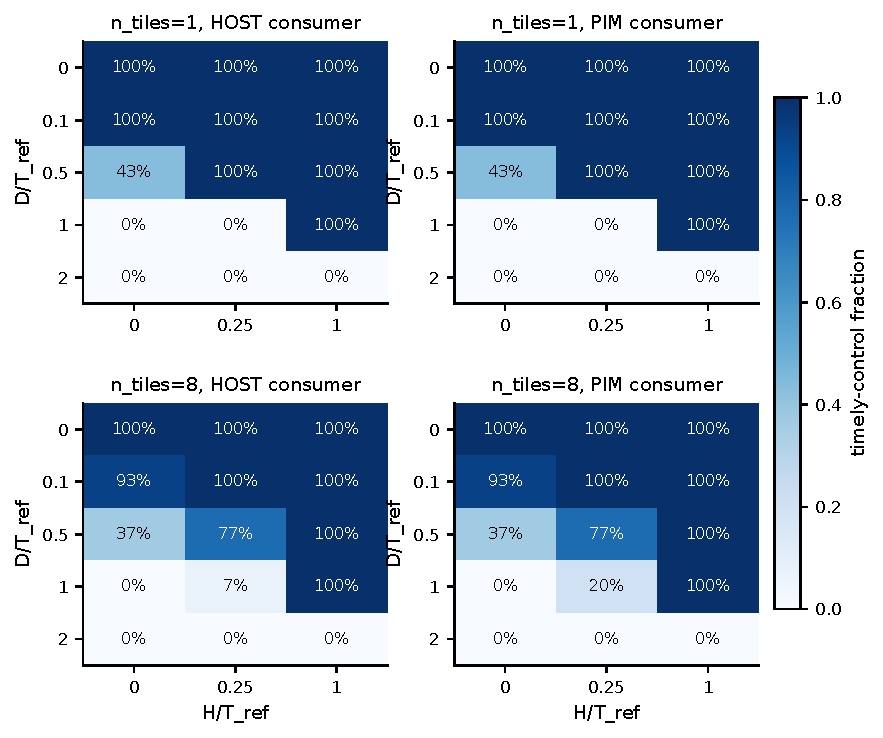
\includegraphics[width=\linewidth]{fig03_control_window.pdf}
\caption{Timely-control fraction for LOCAL\_VISIBLE by consumer and tile
count. Cells are 30 seeds; no main case changed output bits.}
\label{fig:control}
\end{figure}

\subsection{Quiescence}
All 22 P1-D cases ACK without timeout and have zero data-access delta after
ACK. Synthetic quiescence is 1 cycle before submission, 21 cycles with a
nonempty feeder queue, 10/32/66 cycles for in-flight work at K=1/8/32, and
43/65/402 cycles near completion. Actual-CE means are about 13/48/48 cycles.
The two-channel case stops channel 0 (delta 0) while channel 1 advances by 56
accesses; this is not a zero-impact claim. Refresh and the simulator clock
continue through the 8000-cycle observation window.

\begin{figure}[t]
\centering
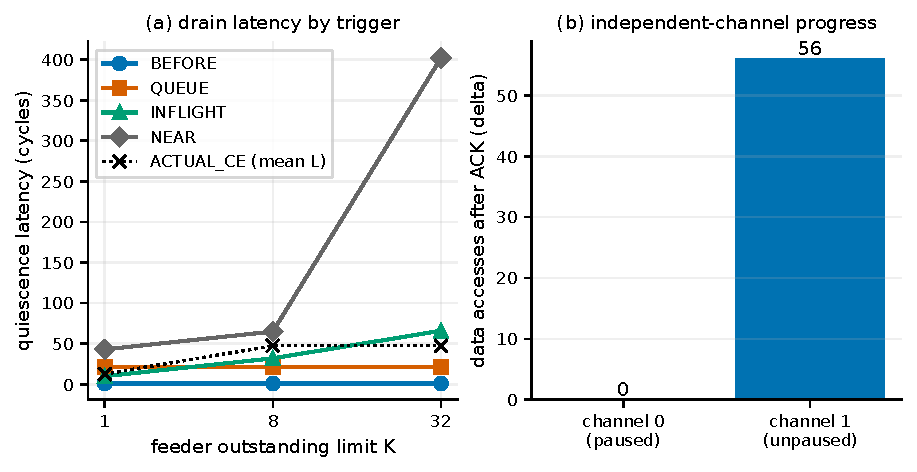
\includegraphics[width=\linewidth]{fig04_quiescence.pdf}
\caption{(a) Quiescence latency by trigger and K; actual CE is a dotted mean
over L. (b) Paused channel 0 versus independent channel 1 progress.}
\label{fig:quiescence}
\end{figure}

\subsection{Trusted-input recovery}
The 20 report-triggered positive cases are all bit-exact after whole-kernel
restart. Table~\ref{tab:restore} gives the deterministic stage costs. The old
output is not published, the old handle becomes stale, and the new version is
published. The seven expected negatives include all five required statuses plus
NO\_INPUT\_RESTORE and NO\_STATE\_RESET.

\begin{table}[t]
\centering
\caption{Recovery stage costs (cycles) and checkpoint size.}
\label{tab:restore}
\begin{tabular}{r r r r r}
\toprule
$n_{\mathrm{tiles}}$ & checkpoint & restore & reexec & ACK$\rightarrow$publish \\
\midrule
1 & 8192\,B & 557 & 804 & 1361 \\
8 & 65536\,B & 4274 & 4130 & 8404 \\
\bottomrule
\end{tabular}
\end{table}

\begin{figure}[t]
\centering
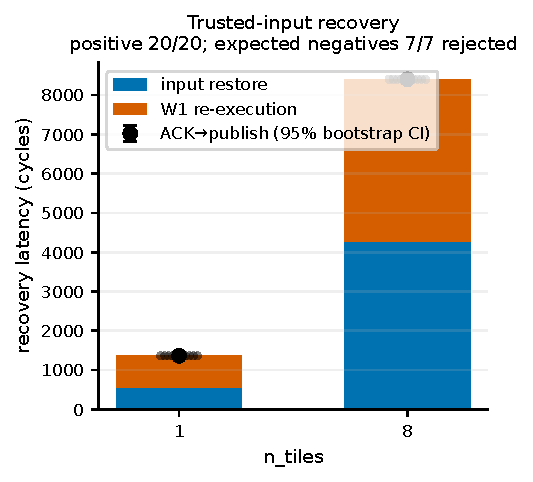
\includegraphics[width=0.62\linewidth]{fig05_restore.pdf}
\caption{Stage decomposition of recovery. Bars are restore and re-execution;
the black marker is ACK$\rightarrow$publish with a 95\% bootstrap interval.}
\label{fig:restore}
\end{figure}

\subsection{Fault-free cost and robustness}
Paired against EXT\_OFF, the mean simulated-cycle overhead is 0.00\% at H0,
10.21\% at H0.25T and 43.96\% at H1T. These are not hardware wall-clock
measurements. H0 costs metadata and held output space but no simulated cycles.
Resident space is 13.6\,KiB at $n_{\mathrm{tiles}}=1$ and 108.1\,KiB at 8,
split into checkpoint, held output, parity and metadata. In robustness, Q=64
delivers all 32 burst reports even at I=64; Q=1 at I=64 delivers 3/32 with 29
queue drops. Drop=0.1 injects exactly three observation gaps at detection
sequence 10/20/30.

\begin{figure}[t]
\centering
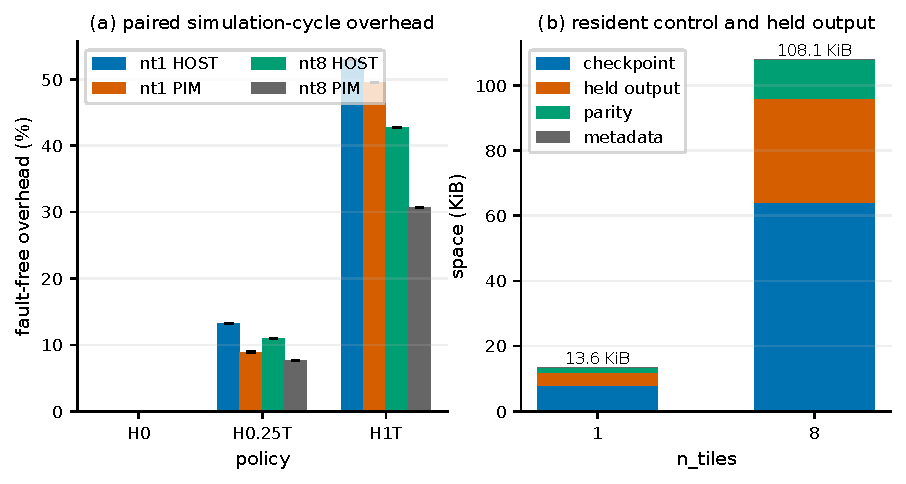
\includegraphics[width=\linewidth]{fig06_cost.pdf}
\caption{(a) Paired fault-free simulation-cycle overhead by policy and
configuration. (b) Resident space components in KiB.}
\label{fig:cost}
\end{figure}

\subsection{P1-G: does timely control stop a corrupted value?}
P1-G uses constructed ECC escapes rather than a corrected single-bit CE. F3M
flips data bits $\{0,1,4\}$: the decoder returns CORRECTED and reports a CE,
but corrects data bit 10 and returns a wrong value. F4S flips
$\{0,1,4,10\}$: the syndrome is zero, the decoder returns CLEAN, and there is
no report. Both modes deliver exactly the same bad 64-bit value. F1W\_F4S adds
a corrected CE witness in one burst and a silent F4S in another, in the same or
a different bank. The evaluator runs only after the case, reads the held B
storage for the corrupt burst, and never gives truth or the corrupt address to
the runtime. PREVENTED requires an unpublished output, a fired runtime lock and
a held B different from the fault-free B. MASKED means FP16 rounding made the
final B/C byte-identical; it is excluded from the control-fraction denominator
and reported separately.

Table~\ref{tab:p1g} gives the n\_tiles=8 HOST panel of Fig.~\ref{fig:escape}.
Across all 4320 P1-G cases, PREVENTED is 2166, CORRUPT\_CONSUMED is 1920 and
MASKED is 234. F3M prevents at small D and/or large H and is consumed when the
report is late; every unmasked F4S case is consumed because there is no report.
The full size/consumer matrix is Fig.~\ref{fig:escape_config}.

\begin{table}[t]
\centering
\caption{P1-G outcomes in the n\_tiles=8 HOST panel (270 cases per
configuration).}
\label{tab:p1g}
\begin{tabular}{lrrrr}
\toprule
configuration & PREVENTED & CORRUPT\_CONSUMED & MASKED & total \\
\midrule
F3M & 172 & 80 & 18 & 270 \\
F4S & 0 & 252 & 18 & 270 \\
F1W\_F4S SAME\_BANK & 180 & 81 & 9 & 270 \\
F1W\_F4S DIFF\_BANK & 180 & 81 & 9 & 270 \\
\bottomrule
\end{tabular}
\end{table}

For F3M, 28 of the 36 Fig.~\ref{fig:control} cells have exactly the same
fraction as TIMELY\_CONTROL; the other eight differ by at most 5.7 percentage
points (3/9 in the n\_tiles=8 HOST panel). Fig.~\ref{fig:control} uses all 30
seeds and classifies TIMELY\_CONTROL from the runtime, whereas P1-G removes
MASKED seeds and additionally requires the held B to be corrupt. The grid
pattern is consistent and the differences are not tuned away. F1W\_F4S
SAME\_BANK and DIFF\_BANK have identical outcomes in 990/1080 matched cases;
the 90 differences are all one side MASKED while the other propagates, never a
case where both propagate and one is prevented while the other is consumed.
DIFF\_BANK has \texttt{report\_covers\_corrupt\_bank=false} in 1080/1080
cases, while SAME\_BANK is true in 1080/1080. The current runtime locks the
whole kernel on the witness CE, so it does not rely on report-region coverage;
a future region-selective recovery would miss the DIFF\_BANK damage.

\begin{figure}[t]
\centering
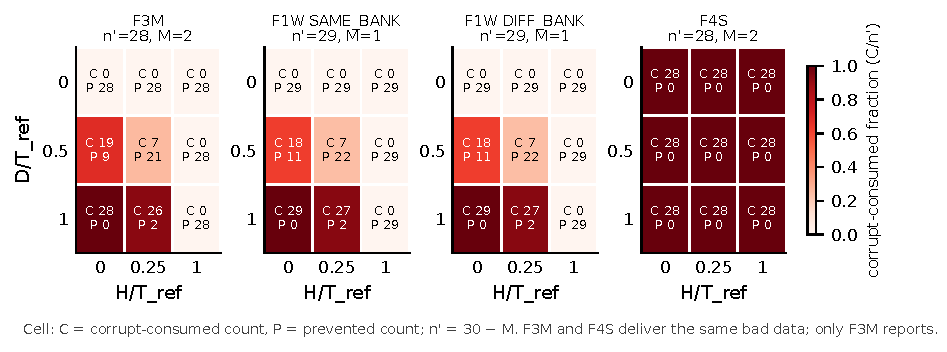
\includegraphics[width=\linewidth]{fig07_escape_efficacy.pdf}
\caption{P1-G escape efficacy for n\_tiles=8 HOST. Color is
CORRUPT\_CONSUMED/$n'$, with $n'=30-\mathrm{MASKED}$; cells show C/P counts
and panel subtitles give $n'$ and MASKED. F3M and F4S deliver the same bad data;
only F3M reports. Constructed patterns, not a Rowhammer probability model.}
\label{fig:escape}
\end{figure}

\subsection{P1-H: what a sequence of coarse reports can distinguish}
P1-H has 330 cases: 10 seeds over six scenarios, bank/page/ASSUMED-codeword
granularity, and with/without ASSUMED idealized scrub. S1 is one persistent bit; S2 is two
independent errors in different codewords of one burst; S3 is the same bank and
a different row; S4 is two susceptible bits in one codeword (dangerous); S5 is
a different bank; S6 repeats the same bit after scrub. Each round reads P, Q,
R in the same order. The public signature is \texttt{error\_class:region\_id}
ordered by \texttt{report\_seq}, excluding \texttt{report\_cycle}.

Table~\ref{tab:p1h} lists the non-singleton 10/10 equivalence groups.
Bank granularity cannot separate dangerous S4 from benign S2, S3 or S6; page
granularity also groups S4 with S2/S5/S6; codeword granularity separates S2 and
S3 from S4 but still cannot separate S4 from S6. Fig.~\ref{fig:ambiguity}
visualizes the pair matrix.

\begin{table}[t]
\centering
\caption{P1-H non-singleton groups with identical report signatures in 10/10
seeds.}
\label{tab:p1h}
\begin{tabular}{llll}
\toprule
scrub & bank & page & codeword \\
\midrule
0 & S2$\equiv$S3 & S2$\equiv$S5 & none \\
1 & S2$\equiv$S3$\equiv$S4$\equiv$S6 &
    S2$\equiv$S4$\equiv$S5$\equiv$S6 & S4$\equiv$S6 \\
\bottomrule
\end{tabular}
\end{table}

The CoF-style rule (fire when one region receives at least two CEs) fires on
S2/S3/S4/S6 at bank granularity, on S2/S4/S5/S6 at page granularity, and on
S4/S6 at codeword granularity (all 10/10 seeds). It fires on S4 but also on
benign scenarios, so it cannot identify S4 by itself. With scrub=0, S4 produces
UE in 10/10 seeds at all three granularities, becoming distinguishable only
after the error is uncorrectable; no other scenario produces UE.
Table~\ref{tab:cof} summarizes the rule.

\begin{table}[t]
\centering
\caption{CoF-style rule at scrub=1: scenarios firing in 10/10 seeds.}
\label{tab:cof}
\begin{tabular}{ll}
\toprule
granularity & firing scenarios \\
\midrule
bank & S2, S3, S4, S6 \\
page & S2, S4, S5, S6 \\
codeword & S4, S6 \\
\bottomrule
\end{tabular}
\end{table}

\begin{figure}[t]
\centering
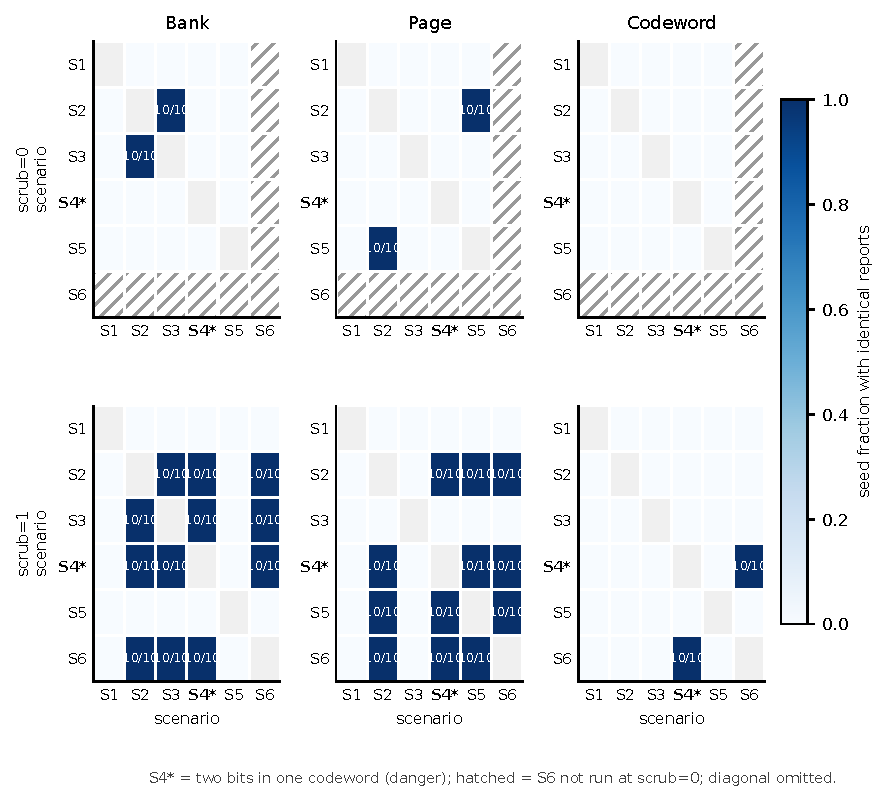
\includegraphics[width=\linewidth]{fig08_report_ambiguity.pdf}
\caption{P1-H report-sequence ambiguity. Rows are scrub off/on; columns are
bank/page/codeword. Color is the fraction of 10 seeds with identical public
report signatures; only non-diagonal pairs are shown, zero cells are blank,
the diagonal is omitted, and hatched cells are S6 at scrub=0 (not run).
S4* is the dangerous same-codeword case.}
\label{fig:ambiguity}
\end{figure}

\begin{figure}[t]
\centering
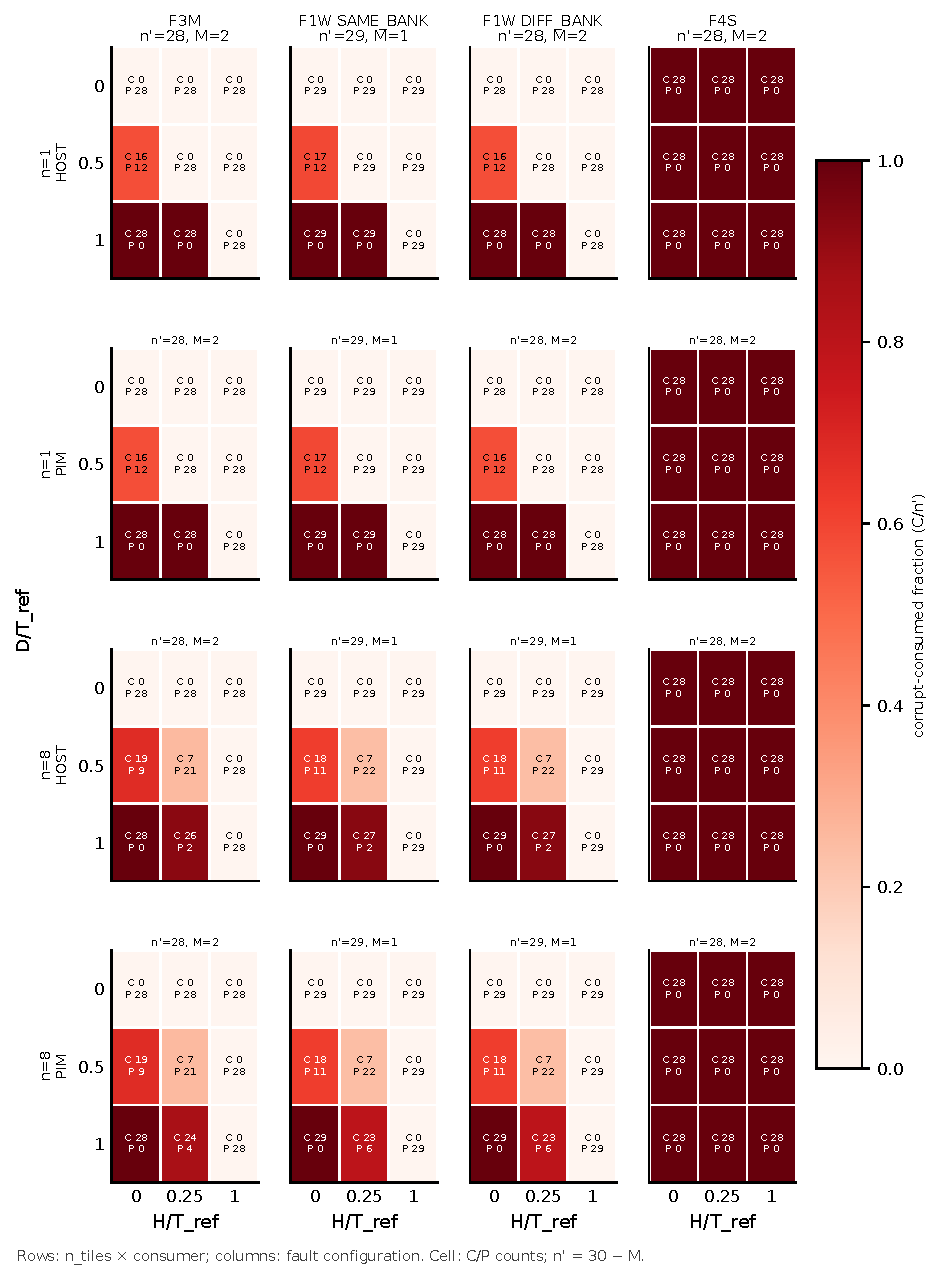
\includegraphics[width=\linewidth]{figS2_escape_by_config.pdf}
\caption{P1-G escape efficacy across n\_tiles and consumer. Rows are
n\_tiles 1/8 by HOST/PIM; columns are F3M, F1W SAME\_BANK, F1W DIFF\_BANK and
F4S. Color and cell text follow Fig.~\ref{fig:escape}; panel subtitles give
$n'$ and MASKED.}
\label{fig:escape_config}
\end{figure}

\section{Expected negatives and failure accounting}
The G8 manifest has 2602 cases: 2595 SUCCESS, 7 EXPECTED\_NEGATIVE, 0 FAIL, 0
TIMEOUT and 0 MISSING. The expected negatives are CHECKPOINT\_MISSING,
VERSION\_MISMATCH, CHECKPOINT\_CORRUPT, ALREADY\_COMMITTED, STALE\_HANDLE,
NO\_INPUT\_RESTORE and NO\_STATE\_RESET. The known upstream
\texttt{PIMBenchFixture.add} score remains 1.98597 $<$ 2.0 and is not counted as
a Phase 1 pass.

Supplement: the independent 4650-case manifest has 4650 SUCCESS, 0 FAIL, 0
TIMEOUT, 0 MISSING and 0 expected negatives. It is reconciled separately from
the paper matrix and is not added to the 2602 count.

\section{Capability judgment}
Within the model, Phase 2 can build on LOCAL\_VISIBLE with bank/page reports, a
bounded queue, output version gating and whole-kernel recovery. The supplement
adds that timely control withholds an actually corrupted constructed escape
output when a report arrives in the same kernel, while a silent F4S without a
report is consumed. The study does not establish that a commercial device
exposes these interfaces, that LOCAL\_HIDDEN reports reach an OS, that
HOST\_ONLY PIM paths are recoverable, or that a persistent Rowhammer attack is
isolated. It also does not establish that coarse bank/page/codeword reports
identify whether multiple susceptible bits share one codeword: P1-H shows that
bank/page cannot separate S4 from benign scenarios and codeword still cannot
separate S4 from S6. The fault is one-shot and recovery does not continue
injection.

\section{Limitations}
The ECC pipeline and energy are not modeled; host copy, interconnect and OS
notification costs are excluded. D, L, H and pause scope are model parameters.
P1-C uses the direct memory path, while P1-F uses the bounded feeder. The
two-channel case uses independent host traffic, not a complete W1/W3 pair.
Drop is a deterministic observation-gap injection. The 30 scenarios are not a
population failure-probability estimate.

The supplement's scrub is an idealized zero-cycle, zero-transaction rewrite;
codeword reporting is an ASSUMED interface; F3M/F4S are constructed CoF-style
patterns, not a Rowhammer probability model. Supplement injections occur once
before the PIM kernel starts; the runtime locks the whole kernel output, not
only the reported region; P1-H uses 10 seeds per (scenario, granularity,
scrub). MASKED is FP16 rounding and is never counted as prevention.

\section{Reproducibility}
The paper matrix is reconstructible from \texttt{scripts/expand\_suite.py},
\texttt{scripts/run\_suite.py}, \texttt{scripts/aggregate.py} and
\texttt{scripts/plot\_paper.py}. The supplement is reconstructible from:

\begin{verbatim}
.venv/bin/python scripts/expand_supplement.py --suite configs/suite_supplement.yaml
.venv/bin/python scripts/run_suite.py --manifest configs/generated/supplement-manifest.json \
    --results-dir results/supplement --runs-dir runs/supplement --jobs 8 --resume
.venv/bin/python scripts/aggregate_supplement.py
.venv/bin/python scripts/plot_supplement.py
\end{verbatim}

The supplement manifest is
\texttt{configs/generated/supplement-manifest.json}; runs are under
\texttt{runs/supplement/} and evidence under \texttt{results/supplement/}.
The smoke manifest is \texttt{supplement-smoke-manifest.json} (24 P1-G +
33 P1-H).

\bibliographystyle{plain}
\bibliography{references}

\end{document}
